%!TEX root = ../thesis.tex
\section{Rehabilitace hlasu po totální laryngektomii}
\label{sec:cause:treatment}

Nesporná výhoda totální laryngektomie neoddiskutovatelně spočívá v likvidaci
primárního nádorového onemocnění. Následky operace však s sebou nesou obrovský
zásah do kvality života pacienta. Okem nejviditelnější změnu představuje
přítomnost tracheostomie a s ní spojený způsob dýchání. Tato skutečnost má
spoustu, na první pohled ne úplně očividných, následků. Postižený člověk
ztrácí přirozené zvlhčování, ohřev a filtraci vdechovaného vzduchu, jež má za
následek vyšší náchylnost k~respiračním onemocněním. Příčina spočívá v
průchodu vzduchu do průdušnice přes tracheostomii a nikoli přes nosní dutiny.

Pro samotného pacienta je však nejspíše nejobtížnější se vypořádat s trvalou
ztrátou vlastního hlasu. Z tohoto důvodu se již samotný autor procedury doktor
Billroth zaobíral otázkou rehabilitace hlasu. Jeho první pokusy s kovovou
tracheostomickou kanylou sice umožňovaly pacientovi hovořit, ale svou
konstrukcí pacienta spíše ohrožovaly na životě \cite{Kramp2009}. Proto se více
uchytila metoda tzv. jícnového hlasu \cite{Sebova-Sedenkova2006}. Ve stejnou
dobu, tedy přibližně začátkem minulého století, se začaly objevovat první
interní a externí hlasové aparáty. V současnosti je rehabilitace hlasu možná
pomocí:

\begin{itemize}
  \item \textbf{foniatrických metod}, mezi které patří jícnový hlas a elektrolarynx,
  \item \textbf{chirurgicko-protetickým způsobem}, který spočívá ve vytvoření kanálku skrze stěnu mezi průdušnicí a jícnem,
  \item \textbf{vytvoření hrtanu podobných struktur chirurgickým způsobem},
  \item \textbf{transplantace hrtanu}.
\end{itemize}

Z uvedeného výčtu se může zdát, že máme k dispozici relativně širokou škálu
možností, jak pacientovi vrátit schopnost vyjadřování pomocí mluvené řeči.
Ovšem je nutné si uvědomit, že je potřeba volit konkrétní metodu podle stavu a
možností pacienta. Jinými slovy, ne každá metoda se hodí pro každého pacienta
a žádná z~metod není univerzální pro všechny pacienty.

\subsection{Foniatrické metody} % (fold)
\label{sub:cause:treatment:foniatric}

Ačkoli odstranění hrtanu vyústí ve ztrátu hlasu, neznamená to, že by byla
úplně eliminována schopnost produkovat řeč. V procesu vytváření hlasu zastává
odstraněný orgán pouze (i když velmi zásadní) roli generátoru zvuku. Zbylé
orgány (hrdelní, nosní a ústní dutina a další) zůstávají nedotčeny a mohou i
nadále plnit svou funkci. Logicky se tak nabízí myšlenka nahradit chybějící
zdroj zvuku jiným. Mezi nejpoužívanější metody patří jícnový hlas a
elektrolarynx.

\subsubsection{Jícnový hlas} % (fold)
\label{ssub:cause:treatment:foniatric:esophageal}

Počátek této metody se datuje do roku 1922, kdy si prof. MUDr. Miloslav Seeman
\cite{seeman1922speech} uvědomil, že funkci štěrbiny mezi hlasivkami (rima
glottidis) přebírá tzv. pseudoglottis, která se vytváří na úrovni horního
jícnového svěrače. Zároveň vypracoval a popsal metodiku vytváření jícnového
hlasu, při které se vzduch neplní do plic, ale do jícnu. Tato metoda se nazývá
\textbf{aspirační}. Princip spočívá v aktivním otevření jícnového svěrače,
nasáváním a vtlačováním vzduchu do jícnu pomocí polykání. Naplněním jícnu
vzduchem si pacient připravuje potřebný vzduch k následné
eruktaci\footnote{eruktace - latinsky název pro proces říhání (popřípadě
krkání), při kterém dochází k úniku plynů pocházejících ze žaludku dutinou
ústní.} vzduchu a produkci řeči. Vlastní jícnový hlas poté vzniká na přechodu
jícnu a hypofaryngu (spodní část hltanu). V této oblasti horního jícnového
zúžení dochází k rozkmitání sliznice a podslizniční vrstvy a produkci zvuku,
který je následně modulován stejně jako v případě přirozené produkce řeči.
Princip tvorby \uv{základního} tónu jícnového hlasu je znázorněn na obr.
\ref{fig:cause:tratment:esophageal}.

\begin{figure}[htb]
  \begin{center}
    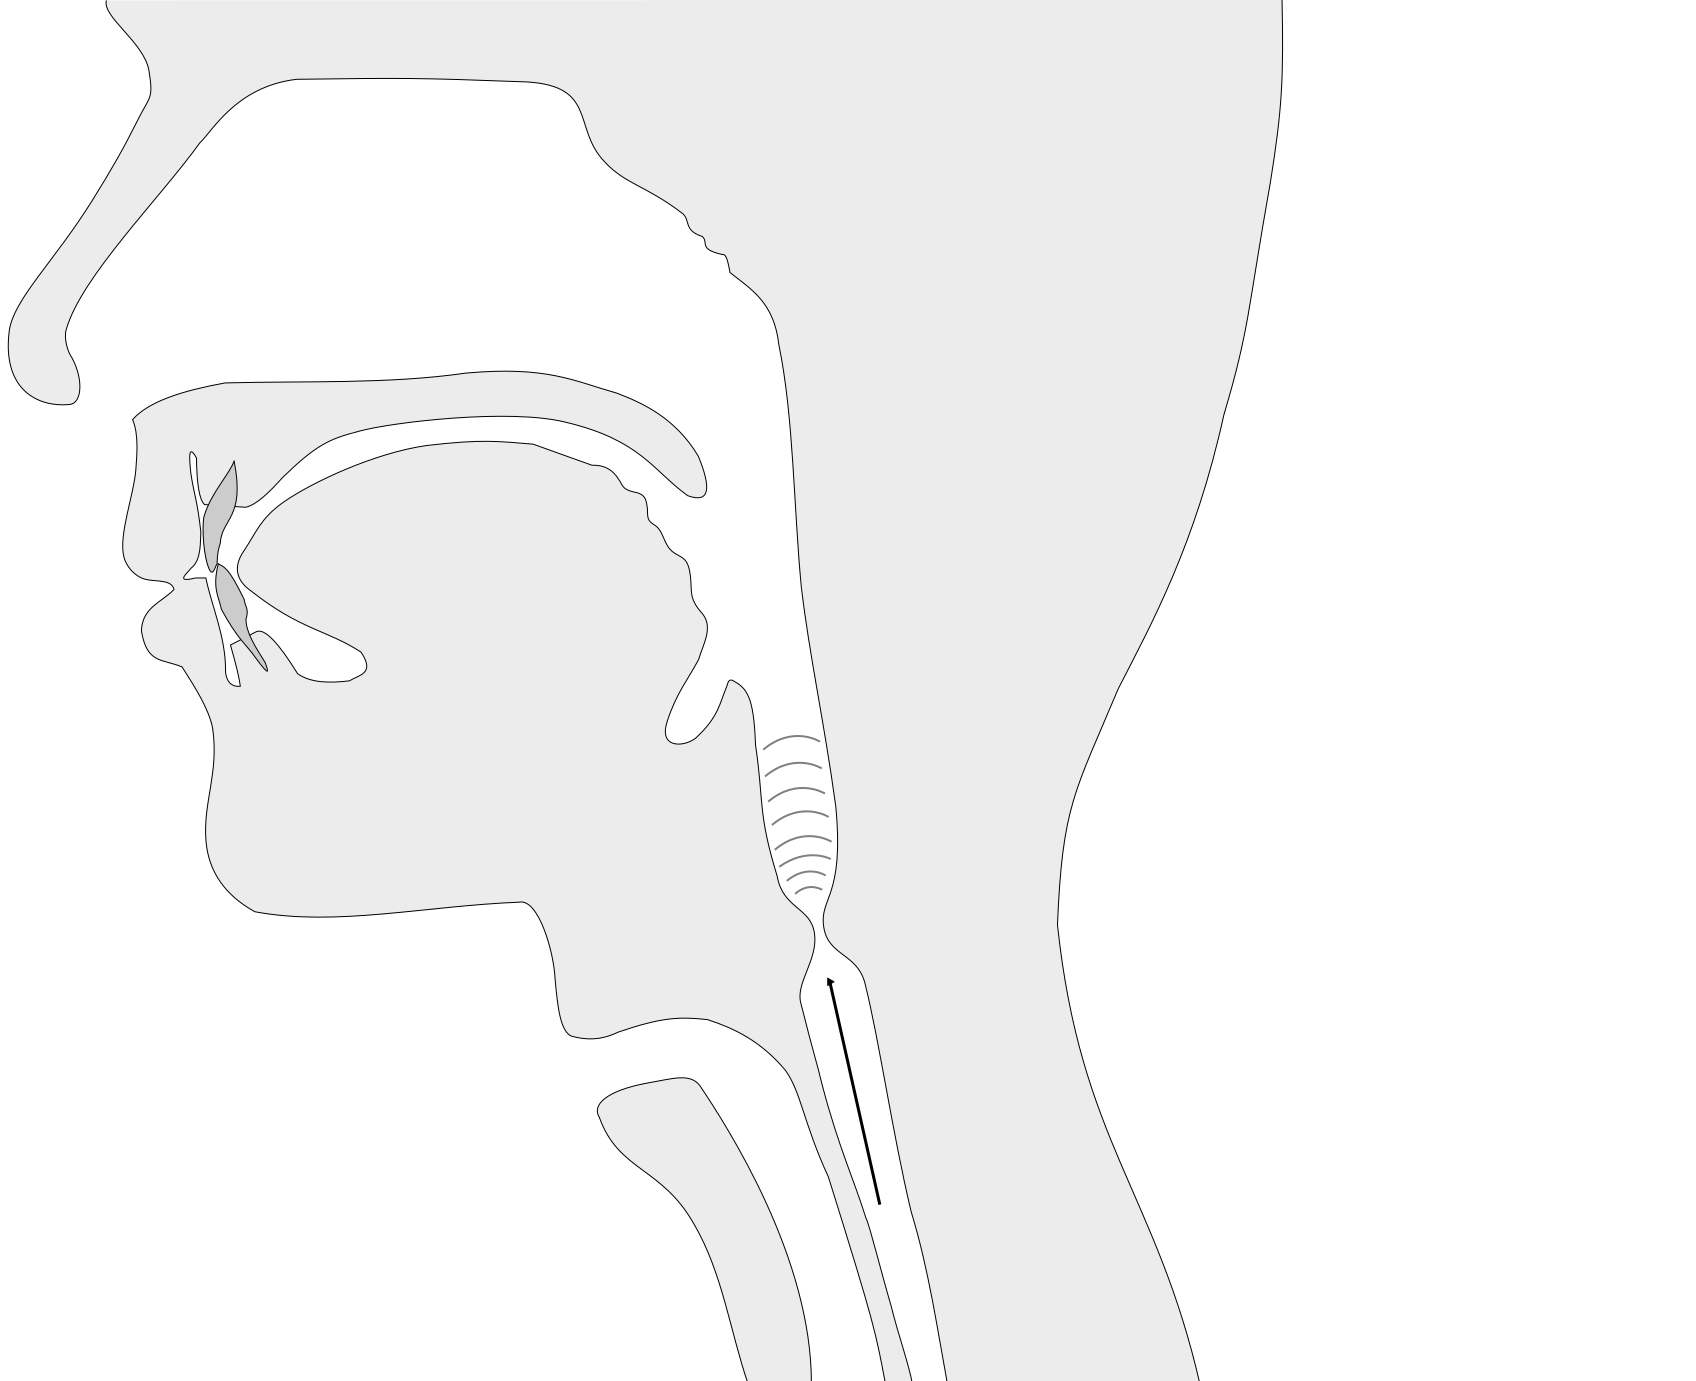
\includegraphics[width=0.6\linewidth]{ch2-cause/figures/esophageal}
    \caption[Princip tvorby jícnového hlasu]{Princip tvorby jícnového hlasu. Průchodem vzduchu přes zúžení vzniká základní tón jícnového hlasu.}
    \label{fig:cause:tratment:esophageal}
  \end{center}
\end{figure}

Kromě aspirační metody je ještě možné se setkat s metodou \textbf{injekční}.
Hlavní rozdíl spočívá v principu plnění vzduchu do jícnu. Při aspirační metodě
se využívá polykání, zatímco v tomto případě je využito kořene jazyka, kterým
je vzduch vtlačován do jícnu. Následný princip produkce hlasu je již shodný s
původní metodou. S tímto principem se můžeme setkat u pacientů, kterým byla
při laryngektomii odstraněna jazylka a aspirační náplň není možná.

Proces učení jícnového hlasu by měl začít co možná nejdříve po operaci. Pokud
je to možné, tak se s výukou začíná ještě za pobytu pacienta na ORL klinice
nebo krátce po propuštění. V první fázi se pacient učí pouze slabiky
sestávající z explosivy a souhlásky. Postupně se však přidávají slabičné
shluky, které sice nedávají smysl, ale pomáhají v osvojení potřebné techniky.
V případě úspěšného zvládnutí se přistupuje k nácviku frází a souvislé řeči.
Potřebnou dobu k nácviku jícnového hlasu nelze přesně určit, protože je
závislá na mnoha faktorech. V literatuře se uvádí, že je potřeba 30 až 50
hodin velmi intenzivního tréninku k osvojení jícnového hlasu.

Míra úspěšnosti nácviku srozumitelného hlasu se uvádí v rozsahu od 14\% do
75\%. Takto obrovský rozsah značí o mnoha faktorech, které mohou ovlivnit
úspěšné osvojení jícnového hlasu. Mezi možné příčiny neúspěchu patří
fyziologické nebo anatomické problémy, psychologické problémy, nebo jednoduše
neadekvátní podpora při řečové terapii \cite{Brown2003}. Velkou roli také
hraje snaha a odhodlání samotného pacienta.

Nepopíratelnou výhodou této techniky rehabilitace je nezávislost pacienta na
lékaři po úspěšném osvojení jícnového hlasu a permanentní oddělení dýchacích a
polykacích cest bez rizika vniknutí potravy do dýchacích cest. Mezi nesporné
výhody také patří volné ruce při vytváření řeči. Za nevýhody se obecně
považuje srozumitelnost produkovaného hlasu. Je to způsobeno jednak
\uv{břišním} zabarvením, které je už z podstaty metody přítomné, a dále také
nízkou intenzitou a krátkou výdrží při tvorbě tónu. Za negativum se dá také
považovat množství pacientem vynaloženého úsilí potřebného k osvojení
techniky. Velmi často se také mluvčí ostýchají jícnový hlas používat, protože
mají pocit, že je společensky nevhodné dorozumívat se formou blízkou říhání. Z
tohoto důvodu se odhaduje, že v běžném životě využívá jícnový hlas pouze 20 až
30\% pacientů, kteří se začali tuto techniku učit \cite{Hradecka2007}.

% subsubsection jícnový_hlas (end)

\subsubsection{Elektrolarynx} % (fold)
\label{ssub:cause:treatment:foniatric:elektrolarynx}

Rehabilitace hlasu pomocí elektrolarynxu se řadí mezi tzv. elektromechanické
metody. Princip spočívá v přikládání zařízení, které obsahuje generátor zvuku
nazývaný elektrolarynx. Přiložením do oblasti spodiny úst a aktivací zařízení
se generovaný zvuk a vibrace přenášejí do dutiny ústní a dalších přilehlých
artikulačních orgánů. Následnou artikulací je pacient schopen hovořit.
Znázorněno na obr. \ref{fig:cause:tratment:electrolarynx}.

\begin{figure}[htb]
  \begin{center}
    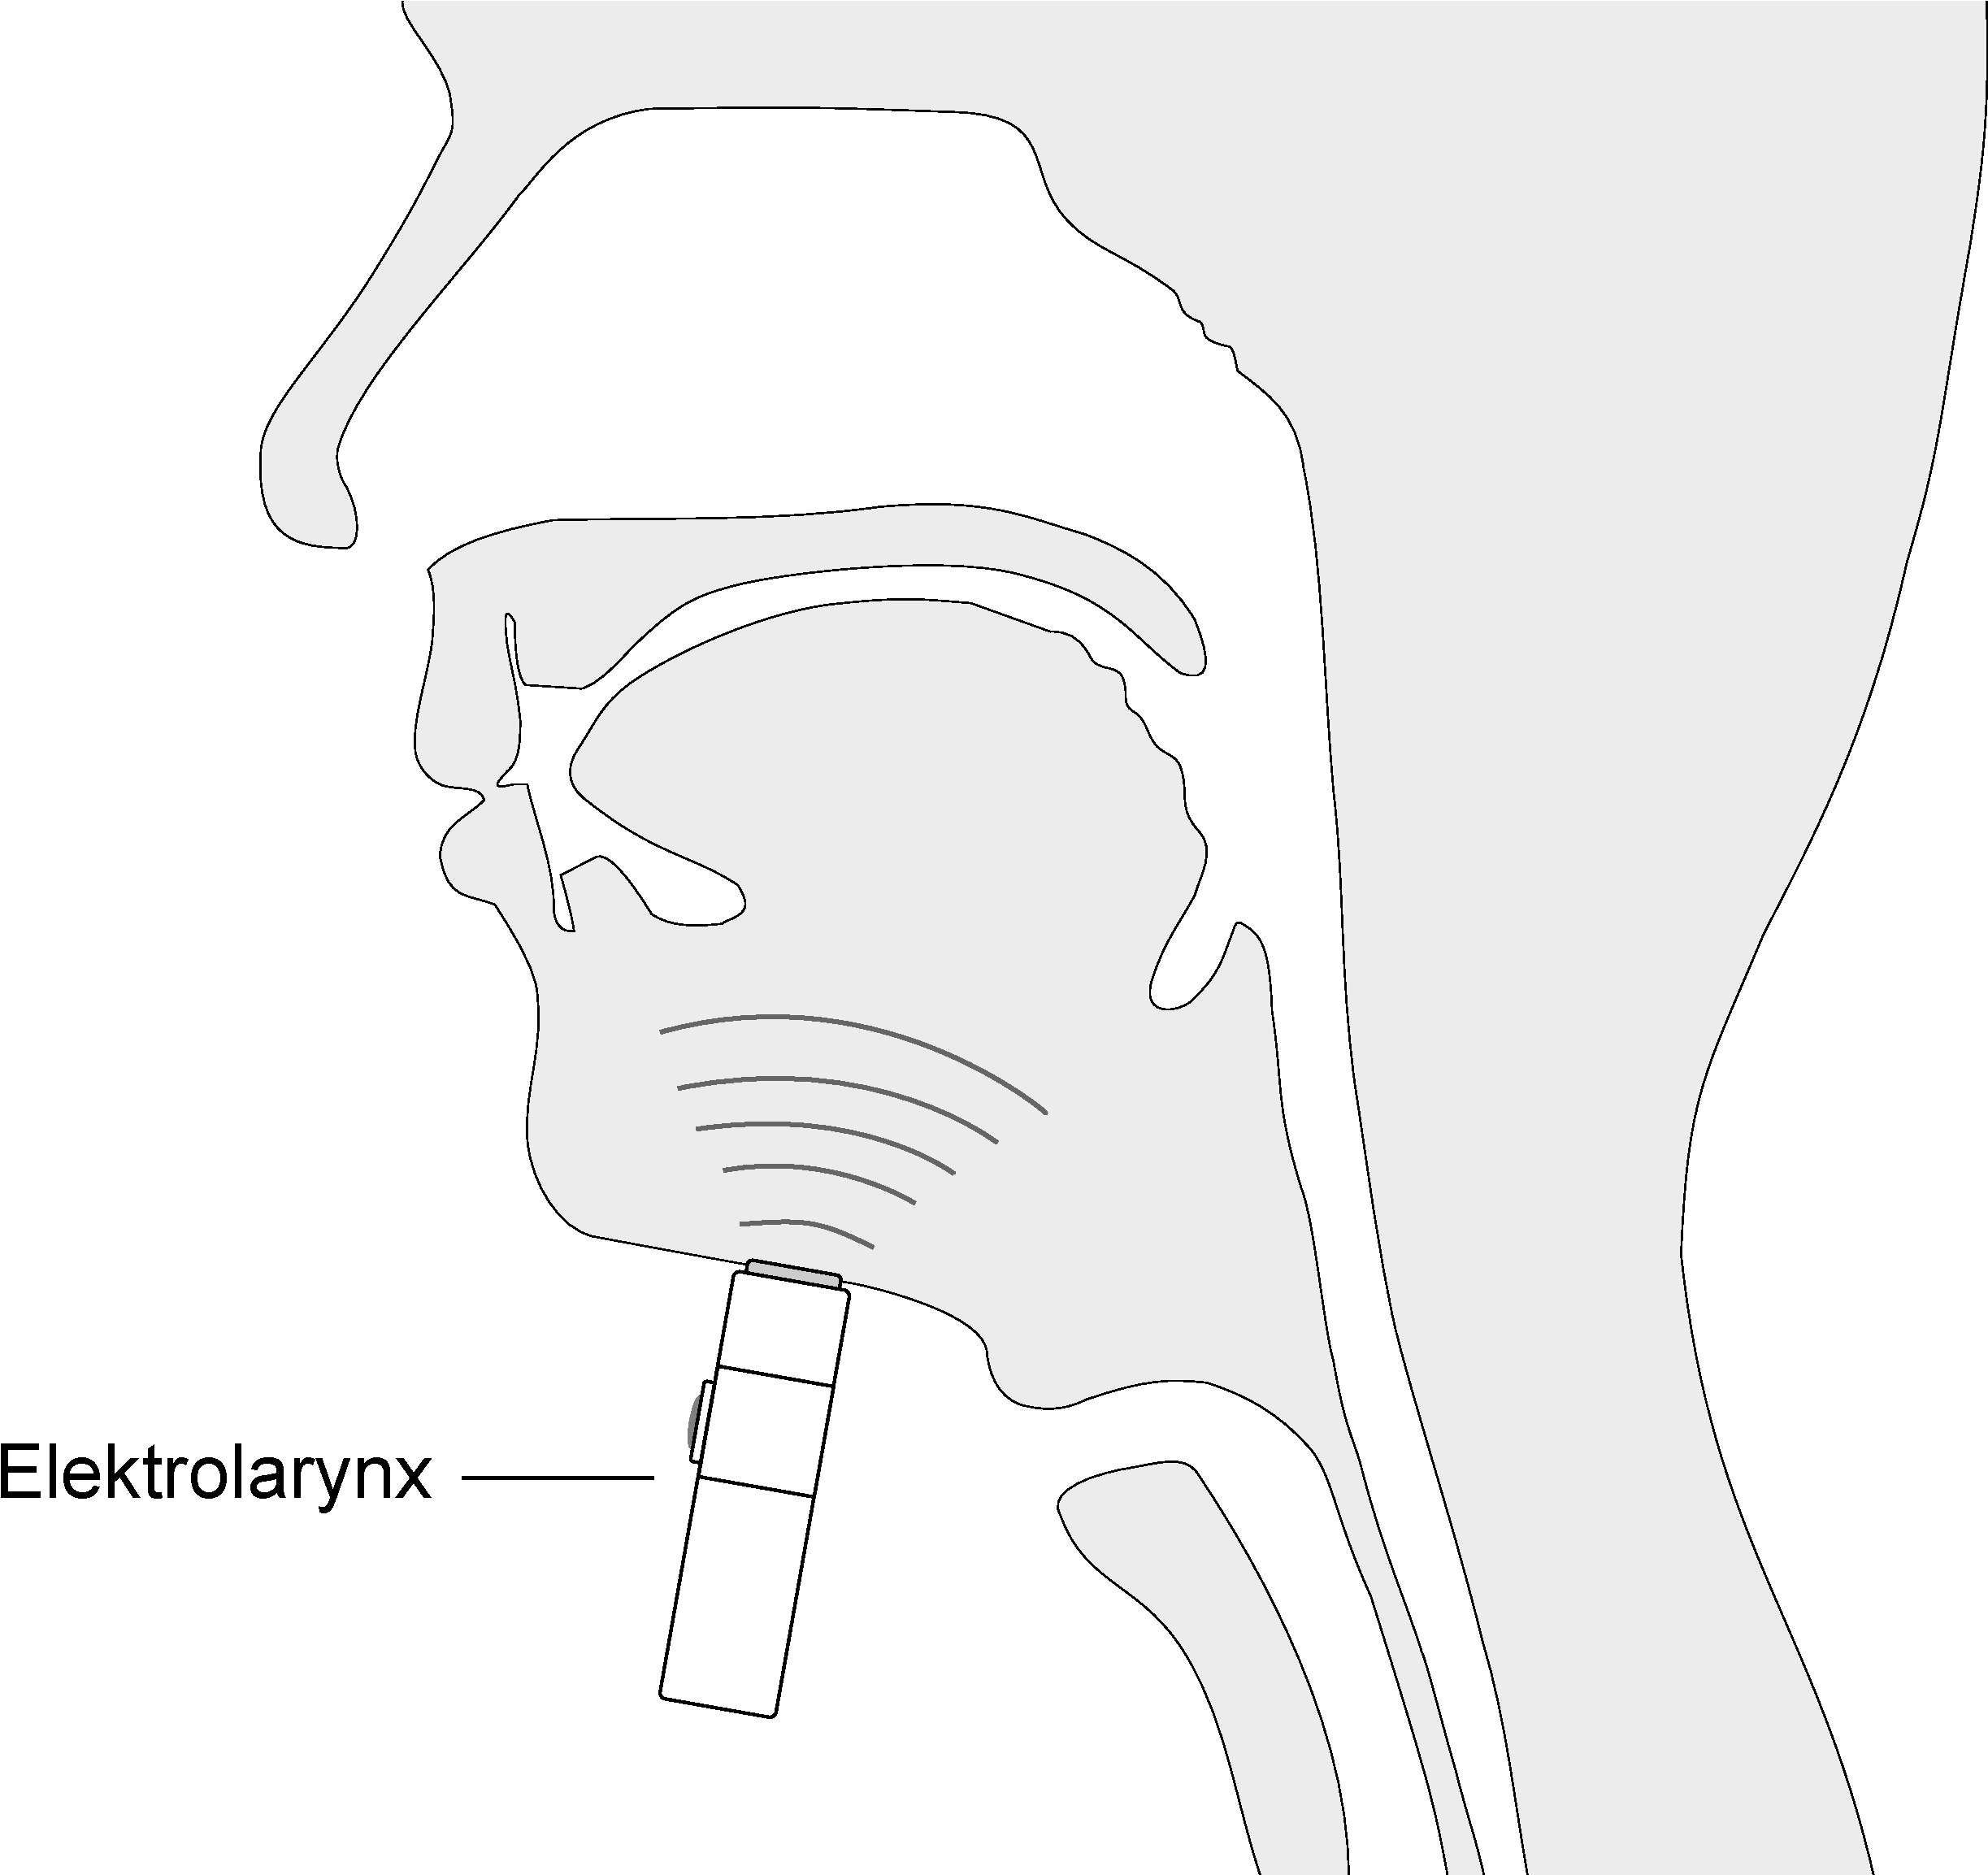
\includegraphics[width=0.6\linewidth]{ch2-cause/figures/electrolarynx}
    \caption[Princip rehabilitace hlasu pomocí elektrolarynxu]{Princip rehabilitace hlasu pomocí elektrolarynxu.}
    \label{fig:cause:tratment:electrolarynx}
  \end{center}
\end{figure}

% TODO: ELEKTROLARYNX pasaze o monotonosti reci poradne promyslet

Takto generovaná řeč se vyznačuje několika charakteristickými rysy. V první
řadě řeč budí velmi mechanický dojem. Důvodem je samozřejmě samotný
elektrolarynx, jelikož se jedná o elektromechanický generátor zvuku s
konstantním buzením, je také základní frekvence produkovaného hlasu více či
méně konstantní. Řečník tak má velmi omezené možnosti, jak řeč emotivně
zabarvovat. V průběhu času se objevily snahy průběžně měnit frekvenci zařízení
a tím ovlivňovat základní frekvenci produkované řeči \cite{Kikuchi2004,
Uemi1994, Goldstein2004}. Hlavním problém všech těchto zařízení je docílit
změnu fundamentální frekvence na základě toho, co chce řečník říci. V současné
době existují pouze experimentální zařízení, která umožňují ve velmi omezené
míře změnu frekvence \cite{Liu2007}. Další charakteristický rys představuje
nižší srozumitelnost řeči, která se ještě snižuje s~rostoucím okolním hlukem.
Velmi často se stává, že posluchač, který se s takto produkovanou řečí setkává
poprvé, není schopen plně porozumět. Se srozumitelností souvisí i další
charakteristický rys, kterým je přítomnost zvukového podkresu produkovaného
samotným přístrojem.

Za hlavní výhodu elektrolarynxu se považuje rychlost osvojení schopnosti
produkovat řeč. Zároveň je tato metoda vhodná pro téměř všechny pacienty
postižené ztrátou hlasu způsobenou léčbou karcinomu hrtanu. Z tohoto důvodu se
hojně užívá u pacientů, kteří si neosvojili jícnový hlas nebo u nich není
možné využití ostatních chirurgických metod.
Za nevýhody se obecně pokládá kvalita produkované řeči, tedy monotonní a
mechanicky znějící hlas. Dále potom zaměstnání jedné ruky držením nebo
spouštěním zařízení.

Samostatnou kapitolou může být psychologický dopad na pacienta. Stejně jako
u~jícnového hlasu se řeč produkovaná promocí elektrolarynxu jeví odlišně od
řeči přirozené. Navíc se ještě přidává potřeba využití nějakého zařízení.
Člověk proto v~mnoha případech cítí ostych a bojí se na veřejnosti mluvit.

% subsubsection elektrolarynx (end)

% subsection subsection_name (end)

\subsection{Chirurgicko-protetická metoda} % (fold)
\label{sub:cause:treatment:tracheo}

Další možnost rehabilitace hlasu představuje tracheoezofageální (zkr. TE) protéza.
První zmínka o vytvoření fistule\footnote{fistule (česky píštěl) je abnormální
otvor mezi dvěma dutými orgány, nebo mezi dutým orgánem a kůží.} mezi
průdušnicí a jícnem pochází z roku 1932. V~tomto roce doktor Guttman poprvé
vytvořil tracheoezofageání shunt\footnote{shunt - kanál, kterým je tekutina
odkloněna z přirozené dráhy. Tento kanál může být vytvořen chirurgicky nebo
pomocí syntetické trubice.} (\uv{umělá píštěl}). Hlavní myšlenka spočívá ve
vytvoření cesty prostřednictvím píštěle, pomocí které u tracheostomovaného
člověka může proudit vzduch z plic do úst. Za normálních okolností vzduch
proudí skrze tracheostomii a do úst se tak nedostane. Zacpe-li si pacient
stomu, může proud vzduchu proudit skrze píštěl do úst. Vzduch procházející
přes fistuli naráží do stěn jícnu a je rozvibrován. Tyto vibrace jsou následně
modulovány pomocí artikulačních ústrojí a tak vzniká řeč.
Tento ojedinělý zákrok otevřel cestu k chirurgické hlasové rehabilitaci.
Vzniklo několik operačních metod, které se navzájem lišili víceméně jen
umístěním fistule \cite{Kramp2009}.

Hlavní snahou chirurgů bylo vytvoření bezpečné, správně nasměrované píštěle
umožňující tvorbu hlasu. Bohužel v mnoha případech byly tyto zákroky spojené
s~vážnými komplikacemi (infekce, zápaly či těžká krvácení). Důležitým
problémem, se kterým se jednotlivý tvůrci museli vypořádat, byla stálost
vytvořeného otvoru tak, aby jím neprotékaly tekutiny špatným směrem a
nedocházelo k zatékání do dýchacích cest a orgánů. Jelikož se jednalo o velmi
náročné techniky, a bylo s nimi spojeno velké množství rizik, došlo v
80.letech 20.století k opadnutí snah tyto metody aplikovat.

Svou renesanci zažily s vložením jednocestného ventilu, který umožňoval pouze
jednosměrný průchod tekutin skrze píštěl, jak je ilustrováno na obr.
\ref{fig:cause:tratment:shunt}. První komerčně dostupná protéza se objevila
v~80.letech 20.století v USA. Na obr. \ref{fig:cause:tratment:prosthesis} jsou
zobrazeny příklady různých typů protéz. Na používané protézy jsou kladené
přísné nároky a musí vyhovovat určitým požadavkům. Předně se musí vyrábět
z~biokompatibilního materiálu, který odolává biodegradaci. Tím je zaručena
dlouhodobá trvanlivost a správná funkce. Potřebný tlak k otevření
faryngoezofageálního segmentu by měl být co nejnižší, aby bylo možné vytvářet
plynulou řeč. První vyráběné protézy měly tento tlak příliš vysoký a omezovaly
tak množinu potencionálních pacientů. Nejmodernější protézy se již vyznačují
velmi nízkým otevíracím fonačním tlakem. V~neposlední řadě by měla být protéza
samofixační a snadno vyměnitelná.

\begin{figure}[htb]
  \begin{center}
    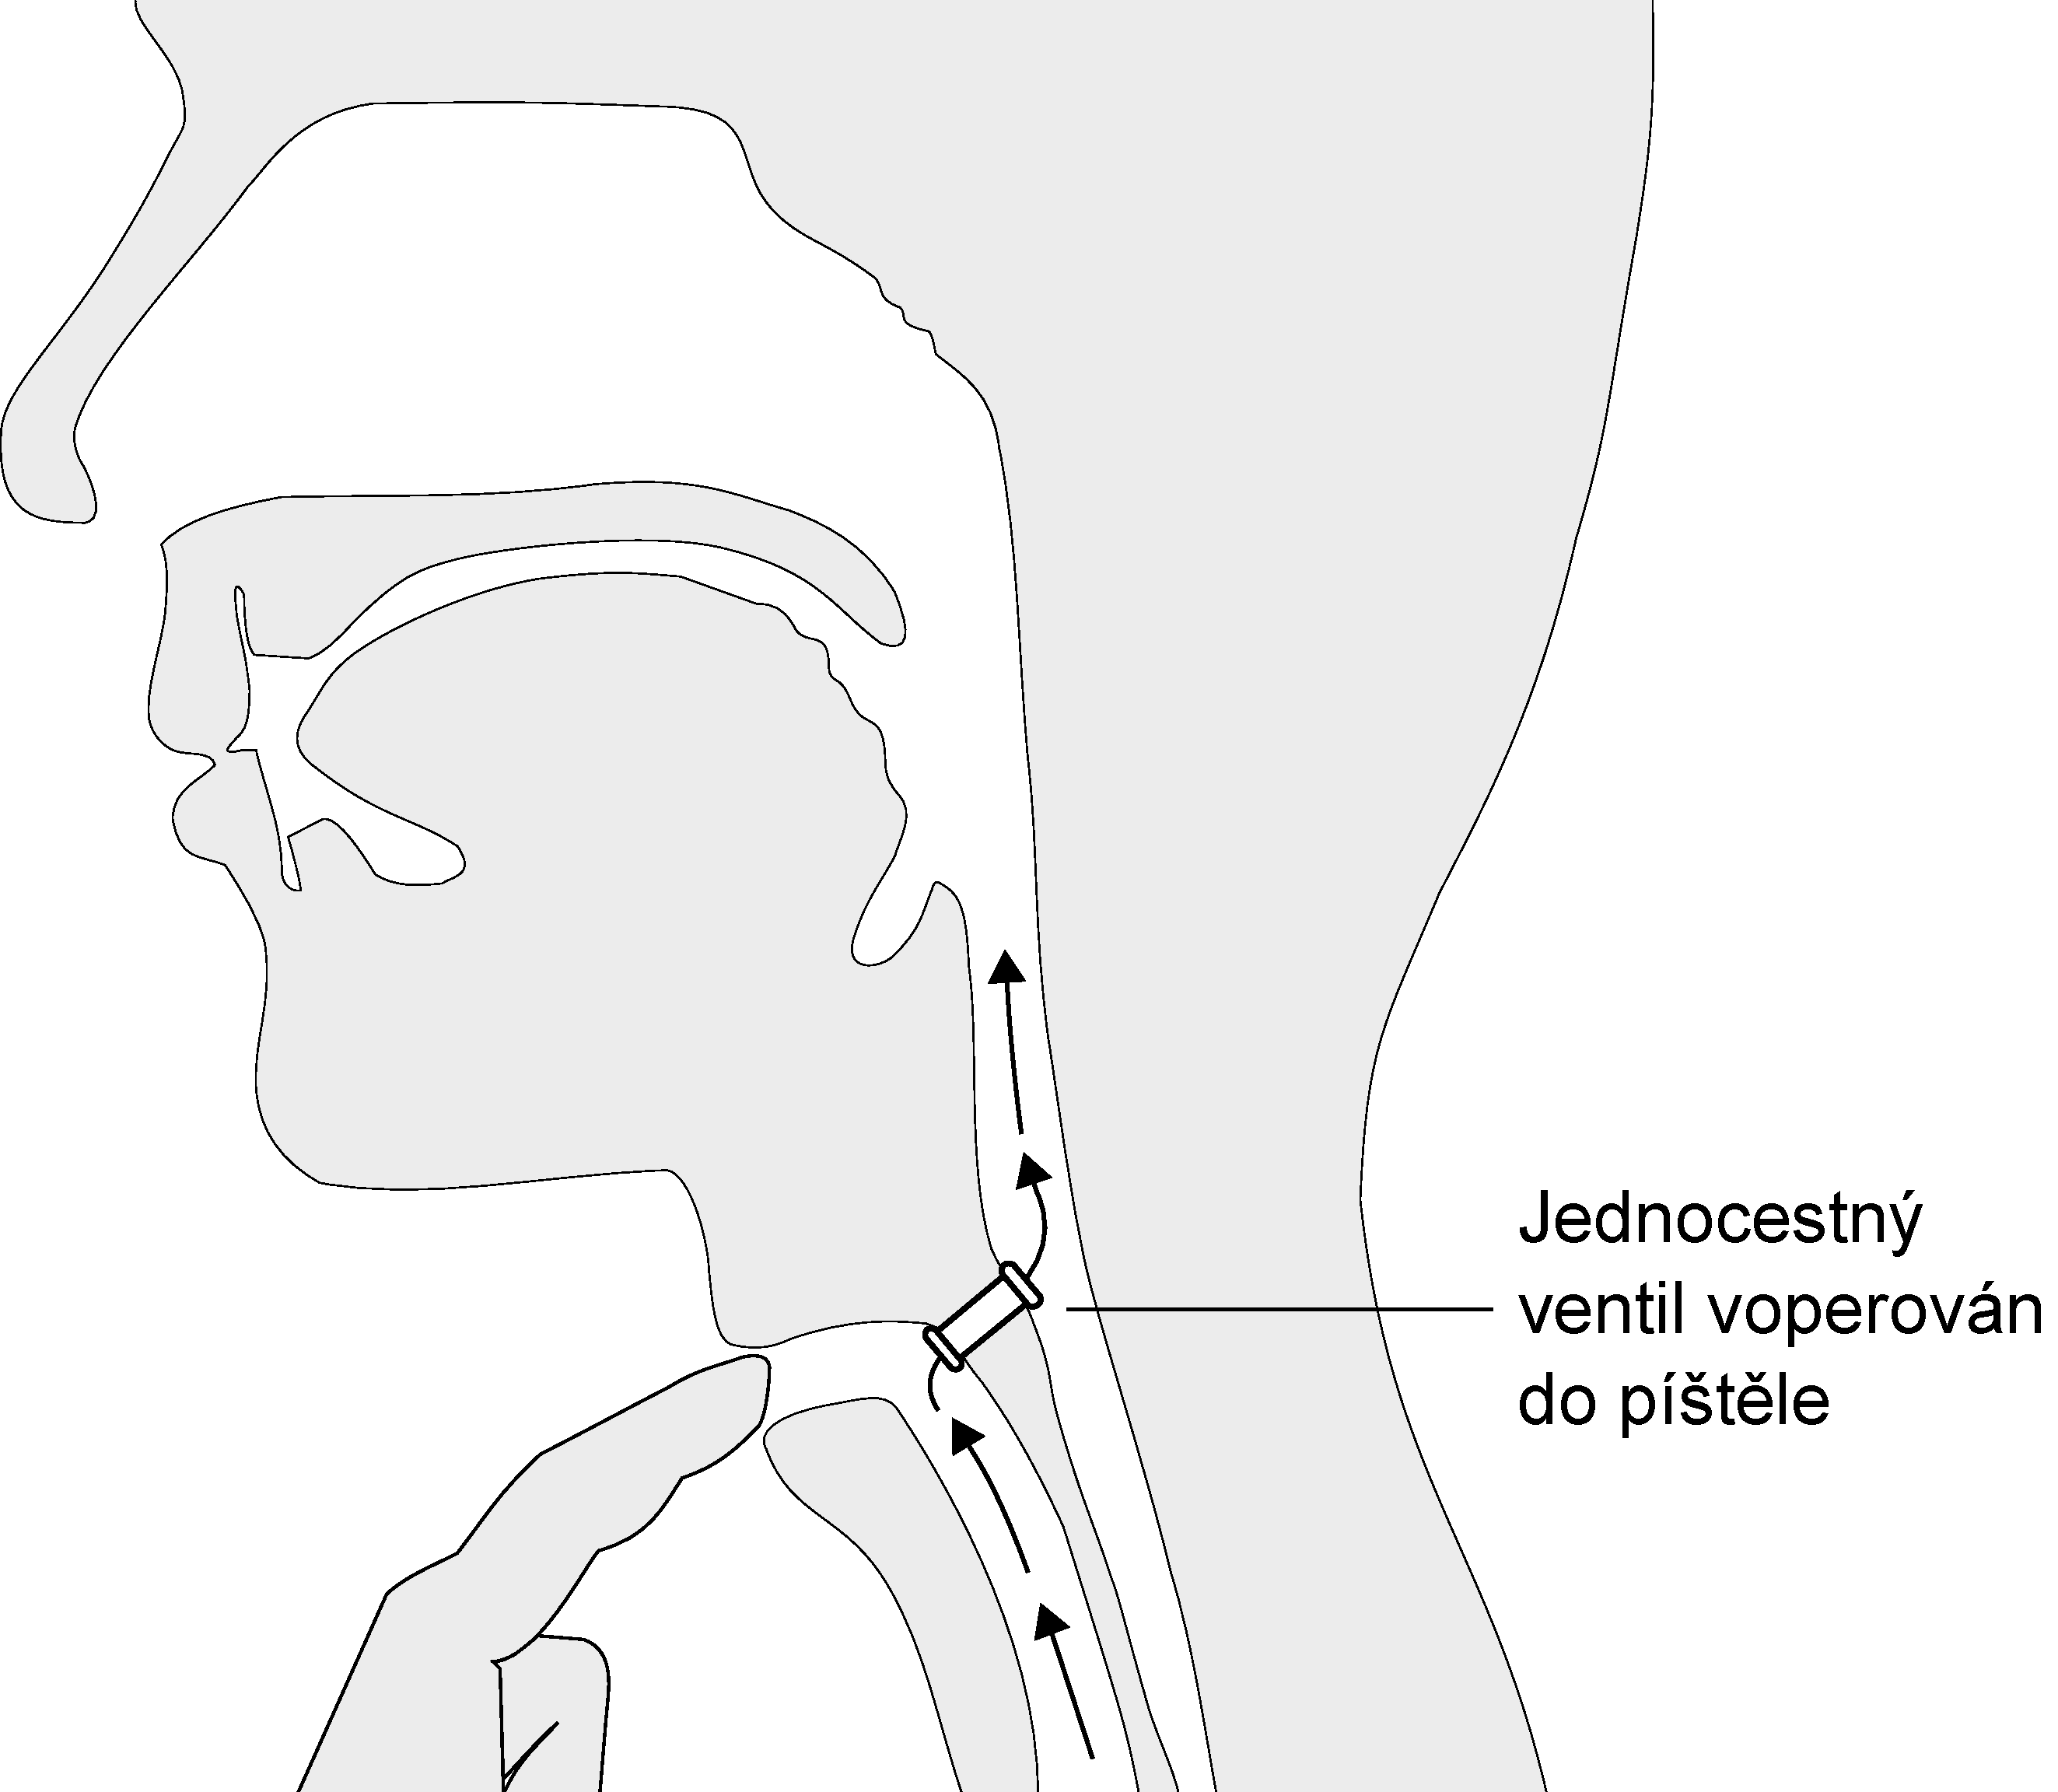
\includegraphics[width=0.6\linewidth]{ch2-cause/figures/te-shunt}
    \caption[Průchod vzduchu tracheoezofageální protézou]{Průchod vzduchu tracheoezofageální protézou.}
    \label{fig:cause:tratment:shunt}
  \end{center}
\end{figure}

\begin{figure}[htb]
  \begin{center}
    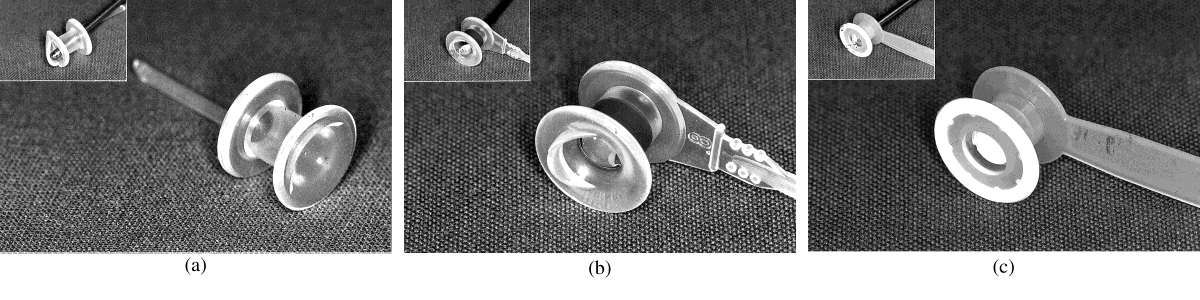
\includegraphics[width=0.9\linewidth]{ch2-cause/figures/te-protezy}
    \caption[Ilustrace používaných TE protéz]{Ilustrace používaných TE protéz (a) Gronigenova nízkotlaká protéza, (b) Provox2 a (c) Blom-Singer protéza.}
    \label{fig:cause:tratment:prosthesis}
  \end{center}
\end{figure}

V praxi se používá několik druhů protéz. Hlavním rozdílem mezi nimi však je
zda se pacient přímo účastní výměny ventilu, jehož fundamentální funkcí je
vytvoření průchodu pro vzduch proudící z průdušnice do jícnu. U protéz, které
jsou vyměňovány operačně, se doba používání pohybuje od 3 do 6 měsíců. Tento
interval velmi významně ovlivňuje tvorba biofilmu na povrchu náhrady. K tvorbě
dochází následkem přímého kontaktu protézy s tělními tekutinami a potravou.
Rychlost tvorby biofilmu ovlivňuje tvar a materiál, ze kterého je náhrada
vytvořena \cite{Leunisse2001}. U typů, které si nositel může měnit sám, se
předpokládá, že budou čištěny nebo měněny přibližně jednou za dva týdny.

Samotný zákrok zavedení protézy je možné provést zároveň s výkonem totální
laryngektomie (tzv. primární zavedení hlasové protézy) nebo až po zotavení
pacienta z~náročné léčby nádorového onemocnění (tzv. sekundární zavedení).
Primární zavedení umožňuje začít s hlasovou rehabilitací krátce po odstranění
hrtanu. Zároveň pacient nemusí v krátké době podstupovat druhou operaci, při
které by se vkládal jednocestný ventil do vytvořené fistule.

V praxi se ukázalo, že úspěšnost rehabilitace je více než 80\%
\cite{Slavicek2002}. Důležitým faktorem, stejně jako u jícnového hlasu, je
funkčnost faryngoezofageálního segmentu. Dále také otvírací tlak horního
jícnového svěrače. Hlas tvořený protézou se vyznačuje vysokou kvalitou, dobrou
srozumitelností, individuálním zabarvením a relativně dlouhou fonační dobou
dosahující průměrně 20 sekund \cite{Saito2003}. Oproti jícnovému hlasu není potřeba
tak intenzivní edukace pacienta k plnému osvojení hlasu. V současnosti se
jedná o nejpoužívanější metodu rehabilitace hlasu.

% TODO: Vyhody nevyhody metody - film tvorici se na proteze
% TODO: Kriteria na pacienta


% subsection chirurgicko_protetická_metoda (end)

\subsection{Hrtanu podobné struktury} % (fold)
\label{sub:cause:tratment:structure}

S rozvojem mikrovaskulárních\footnote{mikrovaskulární - část oběhového systému
složeného z nejmenších cév, jako jsou kapiláry, žilky aj.} transplantátů se
začaly objevovat postupy, které umožňovaly rehabilitovat hlas pouze pomocí
chirurgického zákroku. Tyto techniky umožňují permanentní spojení hypofaryngu
s tracheou pomocí vlastní tkáně pacienta.

První takovouto  metodu představil v roce 1984 doktor Ehrenberger
\cite{Kramp2009}, který popsal tzv. \uv{\textbf{řečový sifón}} (angl. \textbf{speech
siphon}). Tento sifón je vytvořen z části tenkého střeva zvané lačník
(jejunum). Spojení mezi hrtanem a hltanem je dvakrát esovitě zahnuto tak, aby
bylo minimalizováno riziko sekundární aspirace. Schéma \uv{řečového sifónu}
podle Ehrenberga je znázorněno na obr. \ref{fig:cause:tratment:microvascular}
A. Již na první pohled je zřejmé, že se jedná o velmi náročný chirurgický
zákrok. První články publikované autorským kolektivem prezentovaly velmi dobré
funkční výsledky metody. Podle \cite {Sebova-Sedenkova2006} bylo doposud
operováno přibližně 60 pacientů.

V roce 1990 byla popsána laryngoplastika podle Hagena. V tomto případě se
vytváří tzv. \textbf{neolarynx}, k jehož vytvoření se používá štěp z
předloktí. Vnitřek neolaryngu je kryt kůží. Neoglottis je vyztužen chrupavkou
a překrývá vchod do neolaryngu tak, aby nedocházelo k sekundární aspiraci.
Laryngoplastika podle Hagena je znázorněna na obr.
\ref{fig:cause:tratment:microvascular} B. Doposud bylo operováno přibližně 300
pacientů \cite{Sebova-Sedenkova2006}.

\begin{figure}[htb]
  \begin{center}
    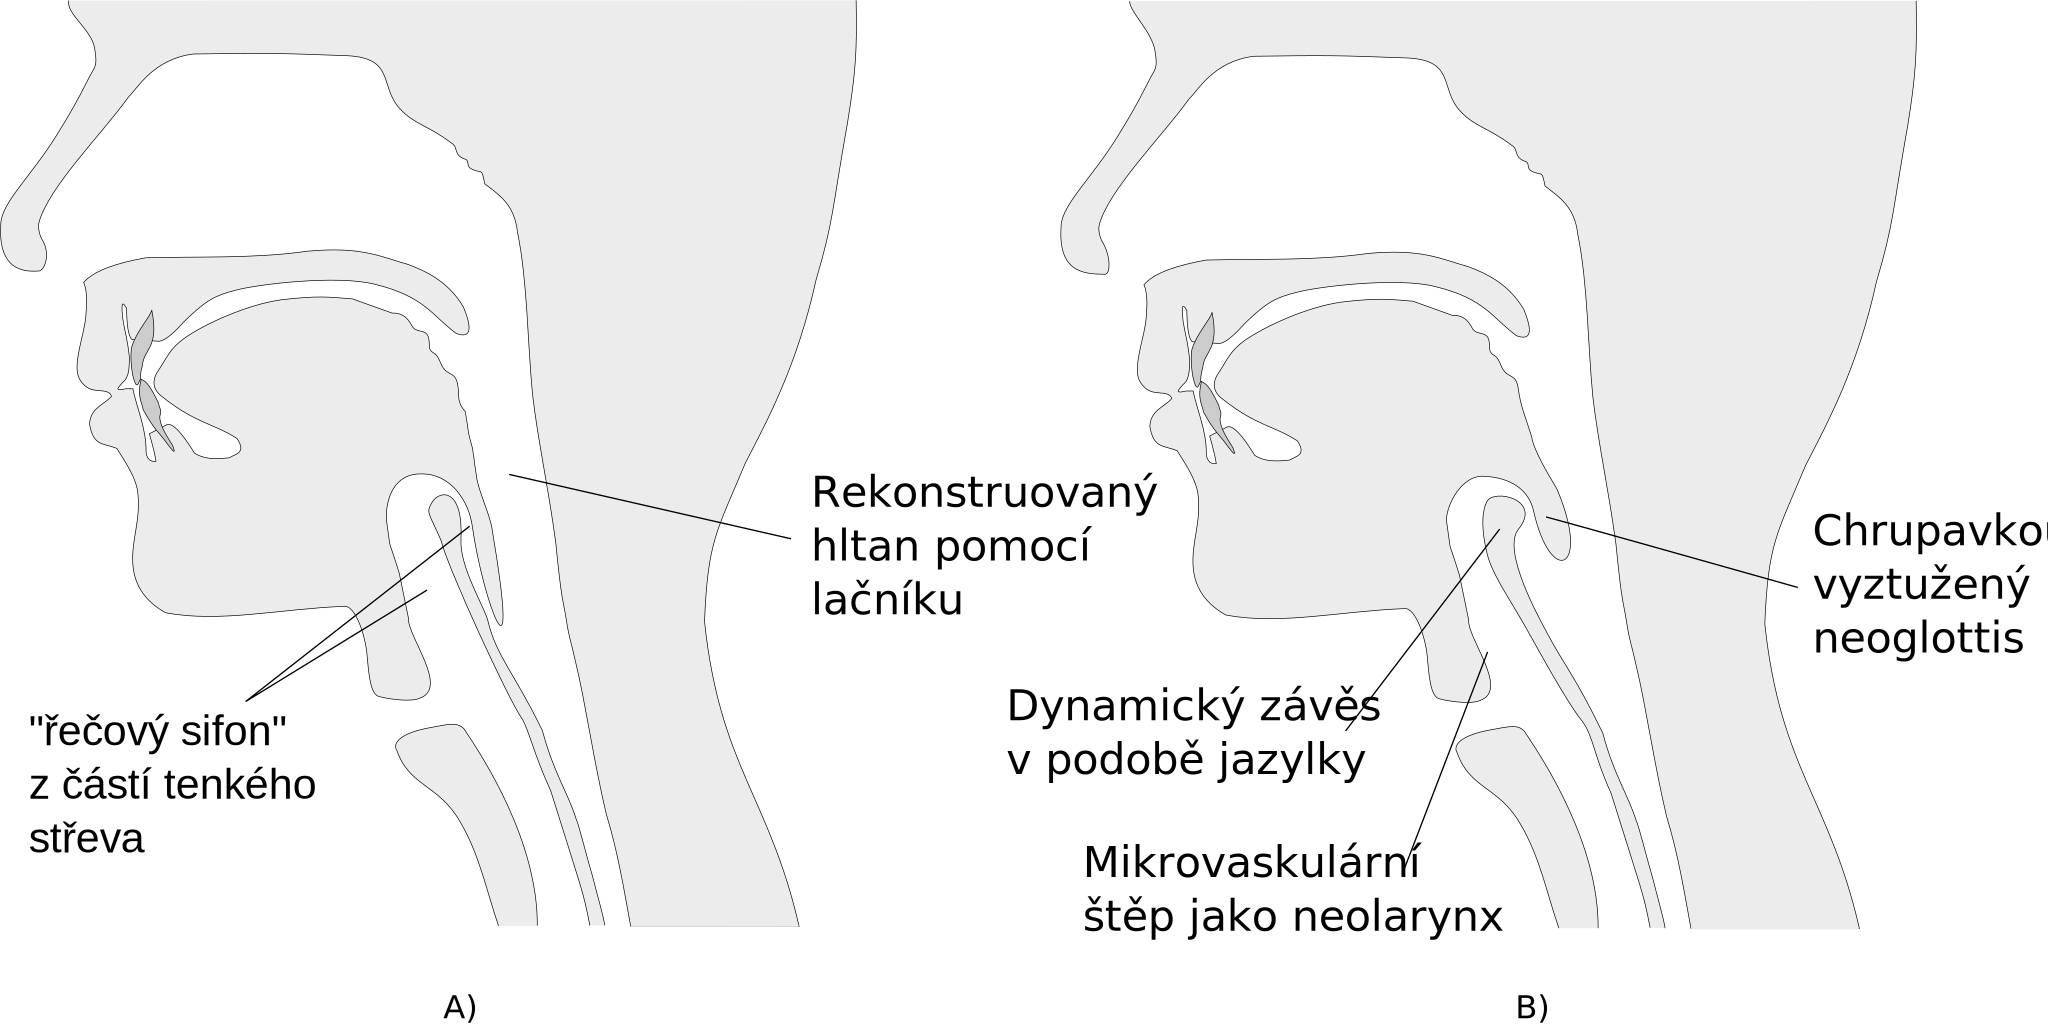
\includegraphics[width=0.9\linewidth]{ch2-cause/figures/microvascular}
    \caption[Schéma \uv{řečového sifónu} a laryngoplastiky]{A) Schéma \uv{řečového sifónu} tak jak jej představil Ehrenberg. B) Laryngoplastika podle Hagena}
    \label{fig:cause:tratment:microvascular}
  \end{center}
\end{figure}

Bohužel v současné době tyto metody nenacházejí širší uplatnění. Především je
to způsobeno chirurgickou náročností samotných metod, kvůli které se velmi
těžko prosazují na dalších pracovištích. Dalším aspektem, který limituje tyto
metody, je vliv na samotného pacienta. Metody předpokládají další chirurgický
zákrok vykonaný po totální laryngektomii. Tento zákrok představuje další zátěž
pro pacienta nemluvě o~možných komplikacích. I přes nedostatky těchto metod je
pochopitelná snaha lékařů o intenzivní výzkum v této oblasti. Při úspěšné
léčbě je pacient schopen produkovat hlas velmi dobré kvality a ve většině
případů nepotřebuje žádnou péči ze strany lékařů ORL.

% subsection hrtanu_podobné_struktury (end)

\subsection{Transplantace hrtanu} % (fold)
\label{sub:cause:treatment:transplantation}

Nejkomplexnější možnost rehabilitace hlasu představuje transplantace hrtanu.
V~tomto případě pacient obdrží implantovaný hrtan od dárce. Pokud je
transplantace úspěšná, přebírá transplantovaný orgán plně funkci původního
orgánu a velmi významně zvyšuje šance pacienta na plné zotavení bez trvalých
následků.

První informace spojené s výzkumem možností provedení transplantace hrtanu se
objevují již v 60. letech 20. století\footnote{Vůbec první úspěšná transplantace
orgánu (ledvin) se uskutečnila v roce 1954.}. Přesto byla první totální
hrtanová transplantace provedena až profesorem Marshallem Stromem v roce 1998
\cite{Narula2011} a do dnešních dnů byly provedeny pouze 2 kompletní
transplantace.

Prvním pacientem, který podstoupil transplantaci, byl čtyřicetiletý muž z USA.
K~laryngektomii v jeho případě vedla motocyklová nehoda, při které si pacient
rozdrtil hrtan. K incidentu došlo 20 let před transplantací. Před zákrokem
používal k~produkci řeči elektrolarynx. Dárcem orgánu byl taktéž čtyřicetiletý
muž, který zemřel na mozkové aneurysma. Úspěch transplantace se na příjemci
projevil již třetí den po operaci, kdy poprvé po 20 letech promluvil (vyslovil
anglické slovo \uv{hello}). Přibližně po 36 měsících od transplantace byl
produkovaný hlas srovnatelný s hlasem zdravého člověka. Podle vlastních slov
pacienta se po operaci jeho kvalita života \uv{nesmírně} zlepšila.
\cite{Strome2001} Doposud poslední úspěšně vykonaná transplantace byla
zaznamenána v~říjnu 2010.

Mezi hlavní důvody takto malého počtu zákroků patří množství pacientů vhodných
pro tuto proceduru. Jelikož se jedná o transplantaci dárcovského orgánu je
nutné použití imunosupresiv, tedy medikamentů zabraňující odmítnutí orgánu.
Imunosupresiva jsou však v současné době nepoužitelná u lidí trpících
rakovinou hrtanu z důvodu velmi vysokého rizika rozšíření rakoviny
\cite{Narula2011}. Další problém představuje náročnost samotného zákroku.
Předně je potřeba provést reinervaci a obnovení krevního oběhu v implantovaném
orgánu. U první provedené transplantace se nepodařilo dosáhnout kompletní
reinervace. Výsledkem tak byl velmi kvalitní generovaný hlas, ale zároveň
nebylo možné pomocí hrtanu zabezpečit bezproblémové dýchání a bylo proto nutné
ponechat tracheostomii.

Poslední výzkum v oblasti imunosuprese však naznačuje, že by v dohledné době
mohlo dojít k pokroku a umožnit transplantaci hrtanu i u lidí trpících
rozsáhlou rakovinou v oblasti krku \cite{Narula2011}. Prozatím je však tato
metoda vhodná pro pacienty netrpící rakovinou, případně ty, u kterých
převažovaly benigní nádory a již 5 let nedošlo k recidivě.

% subsection transplantace_hrtanu (end)

\subsection{Shrnutí} % (fold) \label{sub:treatment:summary}

% NOTE: Neni lepsi pouzit dusledky misto nasledky 3

Rehabilitaci pacientů, kteří prodělali chirurgické odstranění hrtanu, je ve
vyspělých zemích věnována značná pozornost, jelikož následky této operace,
oproti jiným druhům léčby, velmi významně ovlivňují kvalitu života pacientů. V
první řadě se léčený musí vyrovnat se ztrátou hlasu. Tato situace je již sama
o sobě velmi náročnou psychickou zkouškou. Ztráta hlasu je však pouze jedním z
vícero problémů, se kterými je potřeba se vypořádat. Mezi další patří možná
ztráta čichu či vyšší náchylnost k respiračním onemocněním. Neméně významnou
roli sehrává i fyzická odlišnost a z~toho pramenící psychická zátěž pacienta
po absolvované léčbě.

 V současnosti
nejpoužívanějšími metodami rehabilitace hlasu jsou \textbf{tracheoezofageální
píštěl} (popsáno v části \ref{sub:cause:treatment:tracheo}), \textbf{jícnový
hlas} (\ref{ssub:cause:treatment:foniatric:esophageal}) a použití
\textbf{elektrolarynxu} (\ref{ssub:cause:treatment:foniatric:elektrolarynx}).
Existují samozřejmě i další a přehled v současnosti používaných je uveden
v~tab. \ref{tab:treatment:summary}.

\newcolumntype{b}{X}
\newcolumntype{s}{>{\hsize=.5\hsize}X}

\begin{table}[ht]
  \centering
  \begin{tabularx}{1.0\textwidth}{L{1.2} L{0.6} L{1.1} L{1.1}}
    & \textbf{Kvalita} & \textbf{Výhody} & \textbf{Nevýhody} \\
    \toprule \\ [-1.75ex]

    \textbf{Tracheoezofageální píštěl} & Vysoká & Vysoká míra osvojení, dlouhá fonační doba & Zanášení píštěle a s ním spojené čištění, případně dodatečná lékařská péče \\
    \midrule \\ [-1.75ex]

    \textbf{Jícnový hlas} & Dobrá & Volné ruce při mluvení, není potřeba dodatečné lékařské péče & Velmi náročná metoda k naučení, nepřirozený hlas \\
    \midrule \\ [-1.75ex]

    \textbf{Elektrolarynx} & Nízká & Snadné k naučení & Monotonní až robotický hlas, nutné nosit externí elektrické zařízení \\
    \midrule \\ [-1.75ex]

    \textbf{Hrtanu podobné struktury} & Vysoká & Nezávislost pacienta na pravidelné lékařské péči & Velmi náročná chirurgická procedura, která pacienta vystavuje dalším možným rizikům  \\
    \midrule \\ [-1.75ex]

    \textbf{Transplantace hrtanu} & Velmi vysoká & Transplantovaný hrtan přejímá funkci odstraněného orgánu & Velmi náročná chirurgická procedura, která je vhodná jen pro malé procento pacientů \\
  \end{tabularx}

  \caption{Přehled dostupných metod rehabilitace hlasu \label{tab:treatment:summary}}
\end{table}

Většina pacientů je tedy rehabilitována pomocí tracheoezofageálního píštěle,
který principiálně vychází z jícnového hlasu, jehož negativa se snaží
eliminovat. O úspěchu rehabilitace, stejně jako u jícnového hlasu, tak
především rozhodují vlastnosti faryngoezofageálního segmentu. Pokud pacient
není schopen si osvojit jícnový hlas, případně nemá voperován píštěl, je
použit elektrolarynx. Bohužel tyto metody neřeší další problémy spojené s
odstraněním hrtanu, a proto se lékaři stále snaží zdokonalovat rehabilitační
metody. Za nejkomplexnější se dá považovat úplná transplantace hrtanu, která
řeší víceméně všechny problémy spojené s odstraněním hrtanu. Bohužel tento
zákrok je velmi náročný a vhodný pouze pro malou část pacientů.
I když je tedy v současné době lékařská věda schopna rehabilitovat hlas, tak
zde zůstává otevřený prostor pro inovace a tím zlepšení kvality života lidí
postižených ztrátou hrtanu.

% subsection treatment:summary (end)

% section rehabilitace_hlasu_po_totalni_laryngektomii (end)
